\documentclass[a4paper, 12pt, english]{article}

\usepackage[utf8]{inputenc}
\usepackage{amsmath,amssymb}
\usepackage{graphicx}
\usepackage{subfig}
\usepackage[colorinlistoftodos]{todonotes}

\usepackage{indentfirst}
\usepackage{verbatim}
\usepackage{textcomp}
\usepackage{gensymb}

\usepackage{relsize}

\usepackage{lipsum}% http://ctan.org/pkg/lipsum
\usepackage{xcolor}% http://ctan.org/pkg/xcolor
\usepackage{xparse}% http://ctan.org/pkg/xparse
\NewDocumentCommand{\myrule}{O{1pt} O{2pt} O{black}}{%
  \par\nobreak % don't break a page here
  \kern\the\prevdepth % don't take into account the depth of the preceding line
  \kern#2 % space before the rule
  {\color{#3}\hrule height #1 width\hsize} % the rule
  \kern#2 % space after the rule
  \nointerlineskip % no additional space after the rule
}
\usepackage[section]{placeins}

\usepackage{booktabs}
\usepackage{colortbl}%
   \newcommand{\myrowcolour}{\rowcolor[gray]{0.925}}
   
\usepackage[obeyspaces]{url}
\usepackage{etoolbox}
\usepackage[colorlinks,citecolor=black,urlcolor=blue,bookmarks=false,hypertexnames=true]{hyperref} 

\usepackage{geometry}
\geometry{
	paper=a4paper, % Change to letterpaper for US letter
	inner=1cm, % Inner margin
	outer=1cm, % Outer margin
	bindingoffset=.5cm, % Binding offset
	top=2cm, % Top margin
	bottom=2cm, % Bottom margin
	%showframe, % Uncomment to show how the type block is set on the page
}

\usepackage{float}

\usepackage{amsmath,amsfonts}

\usepackage{textcomp}

\usepackage{listings}
\DeclareCaptionFormat{listing}{\centerline#3}
\captionsetup[lstlisting]{format=listing,labelsep=none,justification=justified}

% MATLAB code formatting
\lstdefinestyle{matlab}{
    language=Matlab,
    basicstyle=\footnotesize\ttfamily,
    keywordstyle=\color{blue},
    commentstyle=\color{green!40!black},
    stringstyle=\color{red},
    showstringspaces=false,
    numbers=left,
    numberstyle=\footnotesize,
    numbersep=10pt,
    tabsize=2,
    breaklines=true,
    breakatwhitespace=true,
    captionpos=b
}

% MATLAB command window formatting
\lstdefinestyle{commandstyle}{
    basicstyle=\scriptsize\ttfamily,
    numbers=none,
    showstringspaces=false,
    breaklines=true,
    frame=single,
    frameround=fttt,
    backgroundcolor=\color{gray!10},
    xleftmargin=0.5cm,
    xrightmargin=0.5cm,
    captionpos=b
}
\usepackage{multicol,caption}
\newenvironment{Figure}
  {\par\medskip\noindent\minipage{\linewidth}}
  {\endminipage\par\medskip}
\usepackage{array}

\newcommand{\highlight}[1]{\textcolor{blue}{\texttt{#1}}}

\graphicspath{{images/}}
\setlength {\marginparwidth }{2cm}

%*******************************************************************************%
%************************************START**************************************%
%*******************************************************************************%
\begin{document}

%************************************TITLE PAGE**************************************%
\begin{titlepage}
\begin{center}
\textbf{\LARGE Alexandria University}\\[0.5cm] 
\textbf{\large FACULTY OF ENGINEERING}\\[0.2cm]
\vspace{20pt}

\includegraphics{logo.png}\\[1cm]
\par
\vspace{20pt}
\textbf{\Large EEC471 Automatic Control Systems}\\
\vspace{15pt}
\myrule[1pt][7pt]
\textbf{\LARGE  LABORATORY REPORT 2}\\
\vspace{15pt}
\textbf{\large Design of Satellite-Tracking Antenna}\\
\myrule[1pt][7pt]
\vspace{25pt}
\textbf{\large \hspace{50pt}Student Name \hspace{60pt} Student ID}\\
Ahmed Osama Mohamed Afifi \hspace{60pt} 20010038 \\

\vspace{45pt}
%\textbf {\large Lecturer in charge:}\\[0.2cm]
%\Large {Ir. Chan Cheong Loong}\\[0.1cm]
\end{center}

\par
\vfill
\begin{center}
\textbf{Submission Date : 28/11/2024}\\
\end{center}

\end{titlepage}

%************************************TABLE OF CONTENTS**************************************%

%  %Summary
  %\newpage
  \hypersetup{linkcolor=black}
  \tableofcontents
%  \thispagestyle{empty}
  %End Summary

%********************************%
%***********SECTION 1************%
%********************************%
\newpage
\section{Introduction}
In control systems engineering, understanding and shaping the time-domain response of dynamic systems is crucial for ensuring that systems meet performance specifications such as stability, rise time, overshoot, and settling time. In this lab, two key objectives were explored using MATLAB:

\begin{enumerate}
    \item \textbf{Modeling the system and generating its state-space representation:} The first objective was to model a dynamic system using MATLAB and represent it in state-space form. The equations of motion for the system were derived, converted into a transfer function, and the corresponding state-space representation was generated using MATLAB. State-space modeling is a powerful technique that allows for a comprehensive understanding of the system’s dynamics and facilitates further analysis and design.

    \item \textbf{Analyzing the impact of additional poles and zeros on system performance:} The second objective was to study how the addition of poles and zeros affects the time-domain response of second-order systems. The system's transfer function was modified, and the locations of poles and zeros were adjusted to evaluate their impact on key performance metrics such as overshoot, rise time, and settling time. This analysis is crucial for designing systems that meet specific performance criteria, such as minimizing overshoot or achieving a fast rise time.
\end{enumerate}

The example of a satellite-tracking antenna system was used to demonstrate these objectives, where the elevation of the antenna was regulated using a feedback control law. The system’s dynamics were modeled using the parameters moment of inertia $\left( J = 600,000 kg\cdot{m}^{2}\right)$ and damping coefficient $\left( B = 20,000 M\cdot{m}\cdot{sec}\right)$.
\[J\ddot{\theta} + B\dot{\theta} = {T}_{c} \]
A proportional feedback control law was applied, where the motor torque $\left( {T}_{c} \right)$ was computed based on the difference between the reference angle $\left( {\theta}_{r} \right)$ and the actual angle $\left( \theta \right)$.
\[ {T}_{c} = K\left( {\theta}_{r} - {\theta} \right) \]
where $K$ is the feedback gain.

Throughout the lab, MATLAB was used to:
\begin{itemize}
    \item Generate the state-space model for the closed-loop system.
    \item Analyze the stability and performance of the system for different values of the feedback gain $K$.
    \item Evaluate how changes in the value of $K$ affected key performance metrics like overshoot, rise time, and steady-state error.
    \item Investigate the maximum feedback gain that could be used while maintaining system stability.
    \item Study how the addition of poles and zeros influenced the system’s time-domain response and performance.
\end{itemize}

The work presented in this report highlights the practical application of these control theory concepts, providing insights into how MATLAB can be used to model and analyze the dynamic behavior of control systems.

%********************************%
%***********SECTION 2************%
%********************************%
\newpage
\section{Methodology and Implementation}

This section outlines the methodology used to achieve the objectives of the lab, along with a brief explanation of the MATLAB code, Simulink models, and their corresponding outputs.

%********************************%
%*********SUB-SECTION 1**********%
%********************************%
\subsection{System Modeling} \label{sec:system modeling}

\lstinputlisting[style=matlab, caption=MATLAB code, linerange={12-19}]{"../lab2.m"}

\noindent
The satellite-tracking antenna system was modeled using the given equations of motion:
\[J\ddot{\theta} + B\dot{\theta} = {T}_{c} \]
where:
\begin{itemize}
    \item $J = 600,000 kg\cdot{m}^{2}$ (moment of inertia)
    \item $B = 20,000 N\cdot{m}\cdot{s}$ (damping coefficient)
    \item ${T}_{c} = K \left( {\theta}_{r} - {\theta} \right)$ (control torque).
\end{itemize}

\noindent
The closed-loop transfer function was derived using MATLAB's symbolic computation tools, resulting in:

\[ H(s) = \frac{K}{J{s}^{2} + B{s} + K} \]
This transfer function models the system’s dynamics in terms of feedback gain $K$, and it served as the foundation for subsequent analyses.

\begin{lstlisting}[style=commandstyle,caption=Command line output]]
>> H
 
H(s) =
 
K/(600000*s^2 + 20000*s + K)
\end{lstlisting}

%********************************%
%*********SUB-SECTION 2**********%
%********************************%
\subsection{Generating the State-Space Representation} \label{sec:generating the state-space representation}
\lstinputlisting[style=matlab, caption=MATLAB code, linerange={21-34}]{"../lab2.m"}

For a specific value of $K = 1$, the transfer function was converted to a state-space representation using MATLAB’s \textit{tf} and \textit{ss} functions. This enabled a detailed representation of the system's dynamics. The state-space model is crucial for further control design and analysis, including stability and performance evaluation.

The generated state-space model for $K = 1$ is shown below.

\begin{lstlisting}[style=commandstyle,caption=Command line output]]
>> ss_K1

ss_K1 =
 
  A = 
              x1         x2
   x1   -0.03333  -0.001707
   x2  0.0009766          0
 
  B = 
            u1
   x1  0.03125
   x2        0
 
  C = 
            x1       x2
   y1        0  0.05461
 
  D = 
       u1
   y1   0
 
Continuous-time state-space model.
\end{lstlisting} 

The root locus for $K = 1$ is shown below.

\begin{figure}[H]
    \centering
    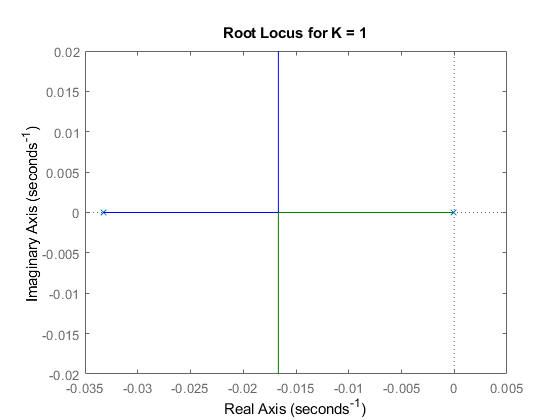
\includegraphics[width=0.7\linewidth]{report/images/RootLocusK1.png}
    \caption{Root Locus for $K=1$}
    \label{fig:Root Locus for K = 1}
\end{figure}

%********************************%
%*********SUB-SECTION 3**********%
%********************************%
\subsection{Stability Analysis} \label{sec:stability analysis}
The stability of the system was analyzed by examining its characteristic equation.
From the closed-loop transfer function, the characteristic equation of the system is given as:
\[ J{s}^{2} + B{s} + K = 0 \]
Divide through by $J$, the normalized form becomes:
\[ {s}^{2} + \frac{B}{J}{s} + \frac{K}{J} = 0 \]
This is a standard quadratic equation of the form:
\[ {s}^{2} + 2{\zeta}{{\omega}_{n}}{s} + {{\omega}_{n}}^{2} = 0 \]
By comparison, the natural frequency ${\omega}_{n}$ and damping ratio $\zeta$ are:
\[ {{\omega}_{n}}^{2} = \frac{K}{J} \quad\mbox{,} {2}{\zeta}{{\omega}_{n}} = \frac{B}{J} \]
Thus, the damping ratio $\zeta$ can be expressed as:
\[ \zeta = \frac{B}{2\sqrt{{J}{K}}} \]
Since $\zeta$  is always positive, the system is inherently stable for all positive $K$ values.

\lstinputlisting[style=matlab, caption=MATLAB code, linerange={36-52}]{"../lab2.m"}

\noindent
To find the maximum $K$ that avoids oscillations, the derivative of $K$ was set to zero.
\[ K = -{J}{{s}^{2}} - {B}{s} \]
\[ \frac{dK}{ds} = -{2}{J}{s} - {B} = 0 \]
Solving for $s$: 
\[s = -{\frac{B}{2J}} \]
Substituting $s$ into the equation for $K$:
\[ K = \frac{{B}^{2}}{{4}{J}} \]
Numerically, this yields $K = \frac{500}{3}$.

\begin{lstlisting}[style=commandstyle,caption=Command line output]]
    >> sln

    sln =

      166.6667

    >> tf_Kmax

    tf_Kmax =
     
               1
      --------------------
      3600 s^2 + 120 s + 1
     
    Continuous-time transfer function.

\end{lstlisting}

\begin{figure}[H]
    \centering
    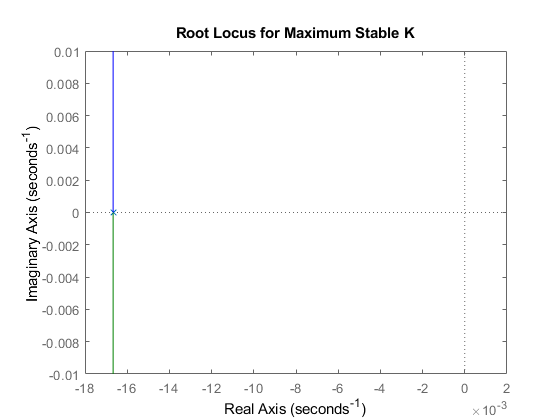
\includegraphics[width=0.8\linewidth]{report/images/RootLocusKmax.png}
    \caption{Root Locus for $ {K}_{max} $}
    \label{fig:Root Locus for Kmax}
\end{figure}

The root locus for the system at $ {K}_{max} $ was plotted (Figure \ref{fig:Root Locus for Kmax}) to confirm the stability condition. The plot shows that the poles, which are two equal real poles, remain in the left half of the complex plane, verifying the stability of the system. This confirms that for $ {K}_{max} $, the system is stable without oscillations, as the poles do not cross into the right half-plane.

\noindent
The analysis shows that while the system is stable for all $ K > 0 $, increasing $K$ beyond $ {K}_{max} $ introduces damping, which may affect the system's transient response. Gains above this value may lead to increased overshoot and reduced damping ratio.

%********************************%
%*********SUB-SECTION 4**********%
%********************************%
\subsection{Overshoot Constraint {$ {{M}_{p}} < {10\%} $}} \label{sec:overshoot constraint}

\noindent
For second-order systems, the percent overshoot ($ {M}_{p} $) is given by:
\[ {{M}_{p}} = \exp{\left( \frac{-{\pi}{\zeta}}{\sqrt{{1}-{\zeta}}} \right)} \times 100\% \]
To ensure that the overshoot is less than $ {10\%} $, the following conditions must be satisfied:
\[ {{\zeta}^{2}} < {1} \quad\mbox{,} \exp{\left( \frac{-{\pi}{\zeta}}{\sqrt{{1}-{\zeta}}} \right)} \times 100\% < 10\% \]
By replacing $ {\zeta} = {\frac{B}{{2}{\sqrt{{J}{K}}}}} $ into the inequalities, we get:
\[ {\frac{{B}^{2}}{{4}{J}{K}}} < {1} \quad\mbox{,} \exp{\left( \frac{-{\pi}{\frac{B}{{2}{\sqrt{{J}{K}}}}}}{\sqrt{{1}-{{\frac{B}{{2}{\sqrt{{J}{K}}}}}}}} \right)} \times 100\% < 10\% \]
Solving these inequalities gives the range of $K$:
\[ {166.6667} < {K} < {476.9205} \]

\lstinputlisting[style=matlab, caption=MATLAB code, linerange={54-75}]{"../lab2.m"}

\noindent
The inequality conditions parameter \textit{ineq.conditions} provides the computed range of $K$ directly from the MATLAB code:

\begin{lstlisting}[style=commandstyle,caption=Command line output]]
    >> ineq.conditions
 
    ans =
     
    x < 8390073680384307/17592186044416 & 500/3 < x
\end{lstlisting}

\noindent
The corresponding range is visualized in Figure \ref{fig:Overshoot constraint}, which shows the valid $K$ values for $ {{M}_{p}} < {10\%} $.

\begin{figure}[H]
    \centering
    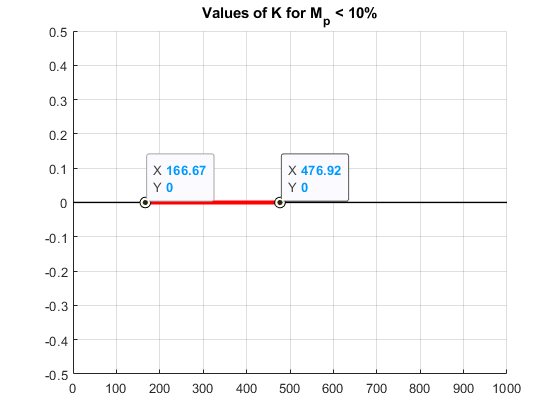
\includegraphics[width=0.8\linewidth]{report/images/KforMp10.png}
    \caption{Range of $K$ for $ {{M}_{p}} < {10\%} $}
    \label{fig:Overshoot constraint}
\end{figure}

Thus, the maximum $K$ for this condition is approximately $ {K} = {476.9205} $, ensuring the system meets the required overshoot constraint.

%********************************%
%*********SUB-SECTION 5**********%
%********************************%
\subsection{Rise Time Constraint {$ {t}_{r} < {80s} $}} \label{sec:rise time constraint}
\noindent
For second-order systems, the rise time $ {t}_{r} $ is given by:
\[ {{t}_{r}} = {\frac{{\pi} - {\theta}}{{{\omega}_{n}{\sqrt{{1} - {{\zeta}^{2}}}}}}} \]
where:
\[ {\theta} = {\arccos\left({\zeta}\right)} \]
To satisfy the condition $ {{t}_{r}} < {80s} $, the following inequalities must hold:
\[ {{\zeta}^{2}} < {1} \quad\mbox{,} {\frac{{\pi} - {\arccos\left({\zeta}\right)}}{{{\omega}_{n}{\sqrt{{1} - {{\zeta}^{2}}}}}}} < 80 \]
substituting for $ {{\omega}_{n}} $ and $\zeta$, we have:
\[ {\frac{{B}^{2}}{{4}{J}{K}}} < {1} \quad\mbox{,} {\frac{{\pi} - {\arccos\left({\frac{B}{{2}{\sqrt{{J}{K}}}}}\right)}}{{\sqrt{\frac{K}{J}}}{\sqrt{{1} - {\frac{{B}^{2}}{{4}{J}{K}}}}}}} < 80 \]

Since solving this inequality analytically is complex, a numerical approach using MATLAB was employed. A binary search was implemented to find the range of $K$ that satisfies these conditions.

\lstinputlisting[style=matlab, caption=MATLAB code, linerange={77-112}]{"../lab2.m"}

The MATLAB output of the inequality conditions parameter \textit{ineq.conditions} provides the computed range of $K$

\begin{lstlisting}[style=commandstyle,caption=Command line output]]
    >> ineq.conditions
     
    ans =
     
    6386945125/16777216 < x
\end{lstlisting}

This result translates to:

\[ {K} > 380.6916 \]

\begin{figure}[H]
    \centering
    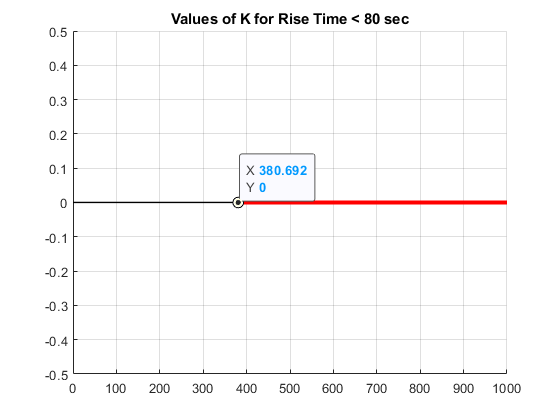
\includegraphics[width=0.7\linewidth]{report/images/KforTr80.png}
    \caption{Range of $K$ for $ {{M}_{p}} < {10\%} $}
    \label{fig:Rise time constraint}
\end{figure}

Thus, the system meets the rise time constraint $ {{t}_{r}} < {80s} $ for all $K$ values greater than approximately $380.6916$.

%********************************%
%*********SUB-SECTION 6**********%
%********************************%
\subsection{Time Response Analysis for Selected Gains} \label{sec:time response analysis for selected gains}
The step response of the system was analyzed for specific feedback gains $ {K} = {\{ 200, 400, 1000, 2000 \}} $ to study the impact of $K$ on overshoot, rise time, and steady-state error.

\lstinputlisting[style=matlab, caption=MATLAB code, linerange={114-137}]{"../lab2.m"}

Figure \ref{fig:Step Response} illustrates the step responses for the selected values of $K$. It can be observed that the system overshoot increases as $K$ rises above the calculated maximum stable $K$ of $166.6667$, consistent with the stability analysis performed earlier.

\begin{figure}[H]
    \centering
    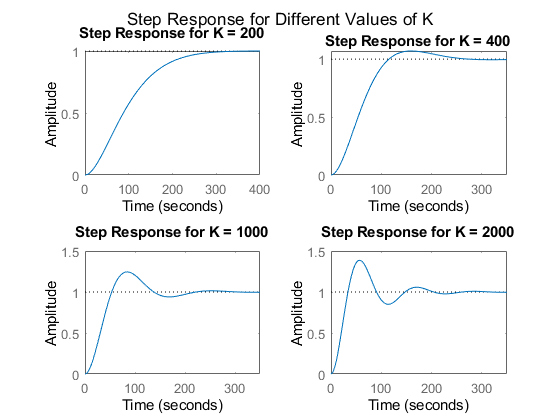
\includegraphics[width=0.8\linewidth]{report/images/stepResponse.png}
    \caption{Step Responses for $ {K} = {\{ 200, 400, 1000, 2000 \}} $}
    \label{fig:Step Response}
\end{figure}

The results for overshoot, rise time, and steady-state error for each value of $K$ are as follows:

\begin{lstlisting}[style=commandstyle,caption=Command line output]]
    For K = 200:
     Overshoot: 0.08893
     Rise Time: 161.1305
     Steady-State Error: 0.5
     
    For K = 400:
     Overshoot: 7.0269
     Rise Time: 76.3235
     Steady-State Error: 0.5
     
    For K = 1000:
     Overshoot: 24.5005
     Rise Time: 36.2328
     Steady-State Error: 0.5
     
    For K = 2000:
     Overshoot: 38.691
     Rise Time: 22.6671
     Steady-State Error: 0.5
\end{lstlisting}

\subsubsection*{Observations}
\begin{enumerate}
    \item \textbf{Rise Time ($ {{t}_{r}} $)}
    \begin{itemize}
        \item The rise time decreases as $K$ increases.
        \item for $K < 380.6916 $, the rise time $ {{t}_{r}} $ falls below $80$ seconds, in agreement with the rise time constraints derived earlier.
        \item Larger values of $K$ result in faster responses (smaller $ {{t}_{r}} $).
    \end{itemize}

    \item \textbf{Overshoot ($ {{M}_{p}} $)}
    \begin{itemize}
        \item Overshoot increases as $K$ grows. This trend is consistent with the overshoot constraint analysis, which predicted increased overshoot for $K$ values exceeding certain threshold $\left( 166.6667 \right)$.
        \item This behavior highlights the trade-off between faster response times (achieved with higher $K$) and increased overshoot, requiring careful selection of $K$ to balance performance criteria.
    \end{itemize}

    \item \textbf{Steady-State Error ($ {{e}_{ss}} $)}
    \begin{itemize}
        \item As the transfer function denominator $ {J}{{s}^{2}} + {B}{s} + {K} $ contains no poles at the origin, the system is classified as \textit{Type 0}.
        \item For a \textit{Type 0} system, the steady-state error for a step input is given by:
        \[ {{e}_{ss}} = {\frac{1}{{1} + {{K}_{p}}}} \]
        where the position error constant $ {{K}_{p}} $ is:
        \[ {{K}_{p}} = {\lim_{{s}\to{0}} {H}\left({s}\right)} \]
        \item Using MATLAB’s \textit{dcgain} function or the formula above, $ {{K}_{p}} = {1} $ for all tested $K$ values, resulting in:
        \[ {{e}_{ss}} = {0.5} \]
        \item Therefore, the steady-state error remains constant at $0.5$ regardless of $K$.
    \end{itemize}
\end{enumerate}
This analysis confirms the interplay between $K$, rise time ($ {{t}_{r}} $), overshoot ($ {{M}_{p}} $), and steady-state error ($ {{e}_{ss}} $), demonstrating that increasing $K$ improves  rise time ($ {{t}_{r}} $) but amplifies overshoot ($ {{M}_{p}} $) while leaving steady-state error ($ {{e}_{ss}} $) unaffected.

%********************************%
%*********SUB-SECTION 7**********%
%********************************%
\subsection{Pole-Zero Analysis} \label{sec:pole-zero analysis for selected gains}
Pole-zero maps were generated for the same selected $K$ values ($ {K} = {\{ 200, 400, 1000, 2000 \}} $) to visualize how the system’s poles and zeros shifted. This analysis provided insights into the system’s dynamic behavior for each gain.

\lstinputlisting[style=matlab, caption=MATLAB code, linerange={139-147}]{"../lab2.m"}

\noindent
In the pole-zero maps for the given gains, as shown in figure \ref{fig:pole-zero map} it is evident that the system has no zeros for all values of $K$  because the transfer function's numerator contains no $s$-dependent terms. However, the system does exhibit two poles, as the denominator is a quadratic function of $s$:
\[ {J}{{s}^{2}} + {B}{s} + {K} \]
The location of these poles depends on the system parameters $J$, $B$, and $K$. For the case of maximum stability $\left( {K} = 166.6667 \right)$, the system reaches its critically damped state, and the poles are located on the real axis with no imaginary component. This is due to the discriminant of the quadratic equation for the poles:
\[ \Delta = {{B}^{2}} - {4}{J}{K} = 0 \]
In this case, the two poles are located at:
\[ {s} = \frac{-B}{2J} \]

\noindent
This corresponds to a critically damped response, where the system will not exhibit any oscillatory behavior, as confirmed in Section \ref{sec:stability analysis}.
For the selected gain values $ {K} = {\{ 200, 400, 1000, 2000 \}} $, he real part of the poles remains the same, at $ \frac{-B}{2J} $, as expected, since the value of $B$ an $J$ do not change. However, as $K$ increases, the imaginary part of the poles increases, leading to oscillations in the system's response, as observed in Section \ref{sec:time response analysis for selected gains}. This is because the discriminant $ \Delta < 0 $, creating complex conjugate poles with non-zero imaginary components. The increased imaginary part leads to the introduction of oscillations, affecting the system's time-domain response.\newline

The pole-zero map provides a clear visualization of these dynamics, where the poles shift as the gain $K$ is varied. As the gain increases, the poles move away from the real axis and towards the complex plane, resulting in a less stable system with increased oscillations. This highlights the importance of selecting an appropriate gain to achieve the desired trade-off between stability and performance.

\begin{figure}[H]
    \centering
    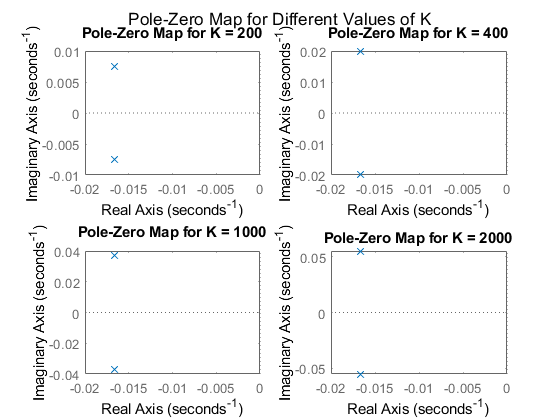
\includegraphics[width=0.8\linewidth]{report/images/pzMap.png}
    \caption{Pole-Zero Map for $ {K} = {\{ 200, 400, 1000, 2000 \}} $}
    \label{fig:pole-zero map}
\end{figure}

%********************************%
%*********SUB-SECTION 8**********%
%********************************%
\subsection{Effect of Additional Poles} \label{sec:effect of additional poles}

\begin{figure}[H]
    \centering
    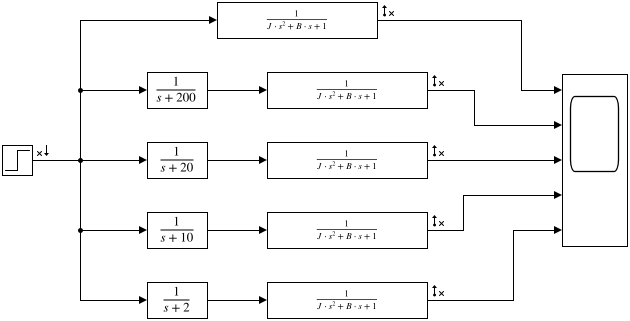
\includegraphics[width=\linewidth]{report/images/poles_step_response_model.png}
    \caption{Simulink model for adding additional poles}
    \label{fig:Simulink additional poles}
\end{figure}

\noindent
To analyze the impact of additional poles on the system's dynamics, a higher-order pole was introduced at $ {s} = {-p} $, modifying the system's transfer function to:
\[ {G\left({s}\right)} = \frac{K}{{\left( {J}{{s}^{2}} + {B}{s} + {K} \right)} {\left( {s} + {p} \right)}} \]
The introduction of the additional pole affects the system's gain and transient response characteristics, but its influence depends on the pole's location relative to the dominant poles.
\begin{figure}[H]
    \centering
    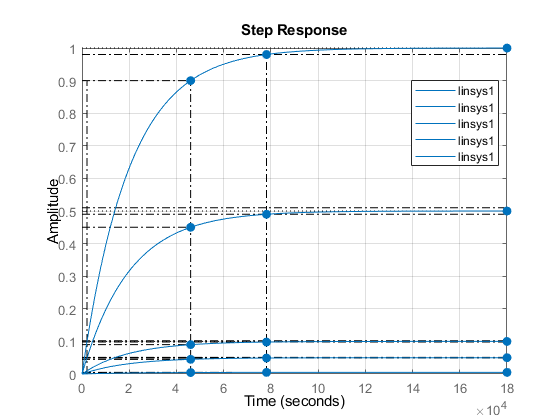
\includegraphics[width=0.82\linewidth]{report/images/poles_step_response.png}
    \caption{Step response for adding additional poles}
    \label{fig:Step response for additional poles}
\end{figure}

\begin{figure}[H]
    \centering
    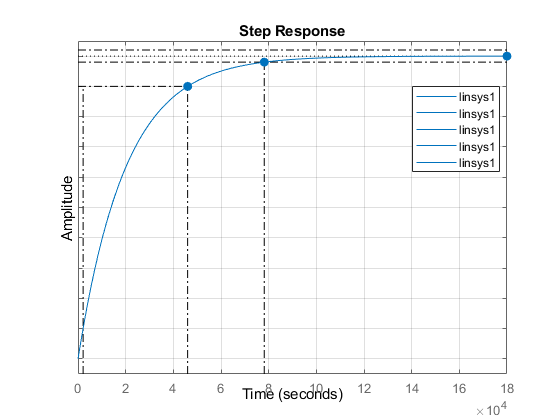
\includegraphics[width=0.82\linewidth]{report/images/poles_step_response_normalized.png}
    \caption{Normalized step response for adding additional poles}
    \label{fig:normalized step response for additional poles}
\end{figure}

\noindent
Figures \ref{fig:Step response for additional poles} and \ref{fig:normalized step response for additional poles} illustrate the step responses for different values of $p$. 
The system dynamics, including rise time, settling time, and overshoot, show minimal variation because the dominant poles, derived from the second-order part of the transfer function $ {J}{{s}^{2}} + {B}{s} + {K} $, primarily dictate the system's behavior.

\lstinputlisting[style=matlab, caption=MATLAB code, linerange={149-180}]{"../lab2.m"}

\begin{lstlisting}[style=commandstyle,caption=Command line output]
    For higher-order pole is nonexistent
     Overshoot: 0
     Settling time: 78153.3784
     Peak time: 210599.9424
     Rise time: 43874.5254
    For higher-order pole at -200
     Overshoot: 0
     Settling time: 78153.3833
     Peak time: 210599.9424
     Rise time: 43874.5255
    For higher-order pole at -20
     Overshoot: 0
     Settling time: 78153.4273
     Peak time: 210599.9424
     Rise time: 43874.5261
    For higher-order pole at -10
     Overshoot: 0
     Settling time: 78153.4762
     Peak time: 210599.9424
     Rise time: 43874.5268
    For higher-order pole at -2
     Overshoot: 0
     Settling time: 78153.8674
     Peak time: 210599.9424
     Rise time: 43874.5322
\end{lstlisting}

Key observations from the data:
\begin{enumerate}
    \item \textbf{Dominant Dynamics Govern Behavior}{\\}
    The system's rise time, settling time, and overshoot are dictated by the dominant second-order dynamics:
    \[ {J}{{s}^{2}} + {B}{s} + {K} = {0} \]
    These dynamics depend only on $J$, $B$, and $K$, which determine:
    \[ \zeta = \frac{B}{2\sqrt{{J}{K}}} \quad\mbox{,} {{\omega}_{n}} = {\sqrt{\frac{K}{J}}} \]
    \item \textbf{Impact of Additional Pole}{\\}
    The additional pole introduces a transient term $ {s} + {p} $, whose contribution depends on the value of $p$:
    \begin{itemize}
        \item Poles located far from the dominant poles decay faster and contribute less to the transient response.
        \item As $p$ approaches the dominant poles, its influence increases slightly, but this is negligible compared to the dominant dynamics.
    \end{itemize}
    \item \textbf{Unchanged Key Metrics}
    \begin{itemize}
        \item \textbf{Overshoot:}
        Determined by the damping ratio $\zeta$ of the dominant poles. Since the additional pole does not alter $\zeta$, overshoot remains unchanged.
        \item \textbf{Rise time:}
        Inversely proportional to $ {{\omega}_{n}} $, which is unaffected by the added pole.
        \item \textbf{Settling time:}
        Inversely proportional to $ {\zeta} \cdot {{\omega}_{n}} $, both of which are independent of the added pole.
        \item \textbf{Peak time:}
        Inversely proportional to the damping frequency $ {{\omega}_{d}} = {{\omega}_{n}} {\sqrt{{1} - {{\zeta}^{2}}}} $. Since $ {{\omega}_{n}} $ and $\zeta$ are unaffected by the added pole, the peak time remains unchanged.
    \end{itemize}
\end{enumerate}

%********************************%
%*********SUB-SECTION 9**********%
%********************************%
\subsection{Effect of Additional Zeros} \label{sec:effect of additional zeros}
\begin{figure}[H]
    \centering
    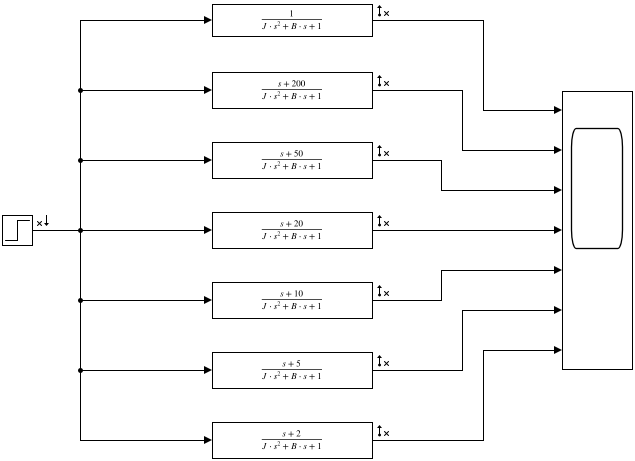
\includegraphics[width=\linewidth]{report/images/zeros_step_response_model.png}
    \caption{Simulink model for adding additional zeros}
    \label{fig:Simulink additional zeros}
\end{figure}
The introduction of a zero at $ {s} = {-z} $ modifies the system's transfer function to:
\[ {G\left({s}\right)} = \frac{{K}{\left( s + z \right)}}{{J}{{s}^{2}} + {B}{s} + {K}} \]
This adjustment impacts the system's response primarily in terms of magnitude scaling at different frequencies, while the dynamics governed by the poles remain unaffected.

\begin{figure}[H]
    \centering
    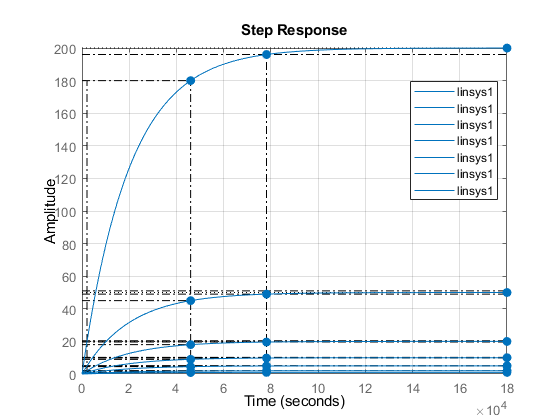
\includegraphics[width=0.82\linewidth]{report/images/zeros_step_response.png}
    \caption{Step response for adding additional zeros}
    \label{fig:Step response for additional zeros}
\end{figure}

\begin{figure}[H]
    \centering
    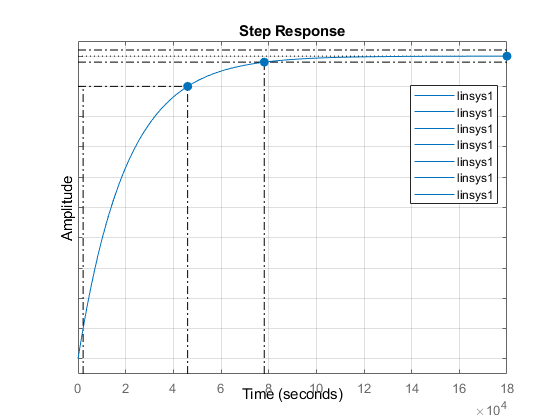
\includegraphics[width=0.82\linewidth]{report/images/zeros_step_response_normalized.png}
    \caption{Normalized step response for adding additional zeros}
    \label{fig:normalized step response for additional zeros}
\end{figure}

\noindent
Figures \ref{fig:Step response for additional zeros} and \ref{fig:normalized step response for additional zeros} illustrate the step responses for different values of $z$.  The system amplitude is affected by the addition of zeros. However, the system dynamics, such as rise time, settling time, and overshoot, remain unchanged as these are governed by the system's poles (which are unaffected by the zero). \newline

\lstinputlisting[style=matlab, caption=MATLAB code, linerange={182-225}]{"../lab2.m"}
\newpage

\begin{lstlisting}[style=commandstyle,caption=Command line output]
    For zero is nonexistent
     Overshoot: 0
     Settling time: 78153.3784
     Peak time: 210599.9424
     Rise time: 43874.5254
    For zero at -200
     Overshoot: 0
     Settling time: 78153.3735
     Peak time: 210599.9424
     Rise time: 43874.5254
    For zero at -50
     Overshoot: 0
     Settling time: 78153.3589
     Peak time: 210599.9424
     Rise time: 43874.5252
    For zero at -20
     Overshoot: 0
     Settling time: 78153.3295
     Peak time: 210599.9424
     Rise time: 43874.5248
    For zero at -10
     Overshoot: 0
     Settling time: 78153.2806
     Peak time: 210599.9424
     Rise time: 43874.5241
    For zero at -5
     Overshoot: 0
     Settling time: 78153.1828
     Peak time: 210599.9424
     Rise time: 43874.5228
    For zero at -2
     Overshoot: 0
     Settling time: 78152.8894
     Peak time: 210599.9424
     Rise time: 43874.5187
\end{lstlisting}

Key observations from the data:
\begin{enumerate}
    \item \textbf{Rise Time, Settling Time, Peak Time, Overshoot}
    \begin{itemize}
        \item These metrics are determined by the dominant poles (roots of $ {J}{{s}^{2}} + {B}{s} + {K} = 0 $).
        \item Since the zero does not alter the poles, these metrics remain unchanged.
    \end{itemize}
    \item \textbf{Influence of the Zero}
    \begin{itemize}
        \item The zero introduces a frequency-dependent scaling term $ \left( {s} + {z} \right) $, which modifies the amplitude of the system's response but does not affect its time-domain characteristics (rise time, settling time, overshoot, etc.).
        \item Zeros farther from the origin cause initial amplification of the system's response. This is because the zero interacts strongly with the high-frequency components of the system.
        \item As the zero approaches the origin, the influence becomes more noticeable in the low-frequency range. This modifies the initial magnitude of the response, but as the zero gets very close to the origin, it begins to have a more subtle effect. The system's behavior is still dominated by the poles, and the zero does not significantly affect the system's time-domain behavior.
    \end{itemize}
\end{enumerate}

%********************************%
%***********SECTION 3************%
%********************************%
\section{Conclusion}
This lab investigated the design and analysis of a satellite-tracking antenna system using MATLAB, with a focus on state-space modeling and the effects of feedback gain, poles, and zeros on system performance. The following key insights were gained:
\begin{enumerate}
    \item \textbf{System Stability and Constraints}
    \begin{itemize}
        \item The system was confirmed to be stable for all positive gain values ($ {K} > {0} $) due to the inherent positivity of the damping ratio ($ {\zeta} > {0} $).
        \item Specific gains were determined to meet performance constraints:
        \begin{itemize}
            \item Critical damping (maximum gain for stability): $ {K} = {166.6667}$
            \item Overshoot constraint ($ {{M}_{p}} < {10\%} $: $ {166.6667} < {K} < {476.9205} $.
            \item Rise time constraint ($ {{t}_{r}} < {80s} $): $ {K} > {380.6916} $
        \end{itemize}
    \end{itemize}
    \item \textbf{Time Response and Feedback Gain}
    \begin{itemize}
        \item Increasing $K$ improved rise time ($ {{t}_{r}} $) but resulted in increased overshoot ($ {{M}_{p}} $), consistent with trade-offs observed in control systems.
        \item Steady-state error ($ {{e}_{ss}} $) was unaffected by changes in $K$, remaining constant at 0.5 for all tested values due to the system’s \textit{Type 0} nature.
    \end{itemize}
    \item \textbf{Effects of Poles and Zeros}
    \begin{itemize}
        \item Adding additional poles far from the dominant poles had negligible effects on system performance metrics (rise time, settling time, and overshoot) due to the dominance of the second-order dynamics.
        \item Introducing zeros influenced the amplitude of the response, particularly at higher frequencies. Zeros closer to the origin modified the system's response at lower frequencies but did not alter time-domain metrics such as rise time or overshoot.
    \end{itemize}
\end{enumerate}

\noindent
This lab highlighted the importance of feedback gain in shaping system performance and emphasized the dominant role of poles in determining time-domain characteristics. The interplay between gain, poles, and zeros underscores the careful consideration required in control design to achieve desired performance metrics while maintaining stability.


\end{document}